El diagrama muestra un triángulo rectángulo y tres cuadrados.
El área del cuadrado más grande es 55 u$^2$, como se muestra en la figura \ref{fig:area11}.

\begin{multicols}{2}
    \begin{figure}[H]
        \begin{center}
            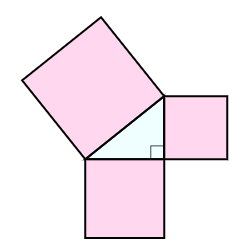
\includegraphics[width=0.4\textwidth]{../images/area11.png}
        \end{center}
        \caption{}
        \label{fig:area11}
    \end{figure}
    \textbf{¿Cuáles pueden ser las áreas de los cuadrados más pequeños?}
    \emph{Marque todas las opciones que considere correctas.}
    \begin{checkboxes}
        \choice $12u^2$ y $38u^2$
        \choice $14u^2$ y $40u^2$
        % \choice $16u^2$ y $37u^2$
        \CorrectChoice $44u^2$ y $11u^2$
        %\choice $5 u^2$ y $11u^2$
        \choice $20u^2$ y $25u^2$
        \CorrectChoice $10u^2$ y $45u^2$
        \CorrectChoice $16u^2$ y $39u^2$
    \end{checkboxes}
\end{multicols}